\documentclass[a4paper,10pt]{article}
\usepackage[utf8]{inputenc}

\usepackage{amstext, amsfonts, amsmath, amsbsy, amssymb}
\usepackage{url}
\usepackage[paper=a4paper,marginparwidth=0mm,marginparsep=0mm,margin=20.5mm,includemp]{geometry}
\usepackage{tikz}
\usepackage{blkarray}
\usepackage[colorlinks=true,linkcolor=blue,anchorcolor=blue,citecolor=blue,filecolor=blue,menucolor=blue,runcolor=blue,urlcolor=black]{hyperref} % For hyperlinks in the PDF
\usepackage[capitalise, noabbrev]{cleveref}

%Math symbols
\DeclareMathOperator{\Exp}{Exp}
\DeclareMathOperator{\Poisson}{Poisson}
\DeclareMathOperator{\Multinom}{Multinom}
\DeclareMathOperator{\logit}{logit}
\DeclareMathOperator{\cov}{cov}
\def\P{\mathbb{P}}
\def\E{\mathbb{E}}

\def\x{\boldsymbol{x}}

\def\btau{\boldsymbol{\tau}}
\def\N{{\cal N}}
\def\M{{\cal M}}
\def\S{{\cal S}}
\def\bmu{\boldsymbol{\mu}}
\def\bxi{\boldsymbol{\xi}}

\linespread{1.25}


%opening
\title{Inferring the presence of metabolites}

\begin{document}

\maketitle

% \section{Model}
%
% 	\subsection{Definition} \label{subsec:definition}
% 	We seek to infer the presence or absence of $M$ metabolites in $S$ species. Let us define a vector of vectors $\vec{v} = \{\vec{v_1}, \ldots, \vec{v_I}\}$ where $\vec{v_i} = \{v_1, \ldots, v_{J_i}\}$ and $J_i$ is the length of vector $\vec{v_i}$. Since we are interested in at least species and metabolites, we expect $I \geq 2$. Hence for this model we expect $\vec{v} = \{\vec{s}, \vec{m}, \ldots\}$ with $\vec{s} = \{s_1, \ldots, s_S\}$ all species and $\vec{m} = \{m_1, \ldots, m_M\}$ all metabolites. Define a vector $\vec{w}$ where $\vec{w} = \vec{v} \hspace{0.5em} \diagdown \{\vec{s}, \vec{m}\}$ of length $K$ with $K = I -2$. Similarly with $\vec{v}$ we have $\vec{w} = \{\vec{w_1}, \ldots, \vec{w_K}\}$ with $\vec{w}_k = \{w_1, \ldots, w_{L_k}\}$.
%
% 	Let us further define $\vec{c}$ a vector containing a single element of $\vec{v_i}$ for each $\vec{v_i}$ in $\vec{v}$. Similarly we have $\vec{b} = \vec{c} \hspace{0.5em} \diagdown \{s, m\}$.  We denote by $x_{\vec{c}} = x_{sm\vec{b}}$ whether metabolite $m$ is present ($x_{sm\vec{b}}=1$) or absent ($x_{sm\vec{b}}=0$) in species $s$ in properties $\vec{b} \in \vec{w}$.
%
% 	We denote $\vec{x}_{s\vec{b}} = (x_{s1\vec{b}}, \ldots, x_{sM\vec{b}})$ the vector of molecules present in properties $\vec{b}$ of a specific species $s$. Finally we define $\vec{x_s} = (\vec{x}_{s1\vec{w}}, \ldots, \vec{x}_{sM\vec{w}})$ the vector of presence/absence of all molecules, for each element of each property, in $\vec{w}$ for species $s$.
%
% 	We assume that related species share a similar set of metabolites and that metabolites related in their synthesis share a similar distribution across species. Let $\P(x_{sm}=1|\mu_m, \epsilon_{sm\vec{b}})$ be the probability with which metabolite $m$ is present in species $s$. We then assume that
%
% 	\begin{equation}
% 	\logit \P(x_{sm}=1|\mu_m, \epsilon_{sm\vec{b}}) = \mu_m + \epsilon_{sm\vec{b}}
% 	\end{equation}
%
% 	where $\mu_m$ is a metabolite-specific intercept and $\epsilon_{sm\vec{b}}$ is normally distributed with mean 0 and co-variance :
% 	\begin{equation}
% 		\cov(\epsilon_{\vec{c}},\epsilon_{\vec{c'}})= \sum_{i=1}^{I} \sum_{d\ne i} \sum_{f=1}^{F} \alpha_{df} \sigma_{c_ic'_i}^{(f)}
% 	\end{equation}
%
% 	with $I$ the length of vector $\vec{v}$ (or $\vec{c}$), $\sigma$ a known measure of covariance and $\alpha$ a positive scalar. $\sigma_{c_ic'_i}^{(f)}$ is defined as a known measure of covariance between property $c_i$ and $c_i'$ when looking at feature $f$. $f$ being a feature at which the variance is measured. For example, this would allow to discriminate the variance of two species when looked at the "phenotype", or "environment" level or any arbitrary feature one is interested in.
%
%
% 	\subsubsection{Updating parameters}
%
% 	To update our parameters using Metropolis-Hastings algorithm, we need to propose a suitable ration $h$ for each parameter to be updated. We know that :
%
% 	\begin{equation}
% 		P(\vec{\alpha} | \vec{x_s}, \vec{\mu}) \propto P(\vec{x_s} | \vec{\mu}, \vec{\alpha}) P(\vec{\alpha})
% 	\end{equation}
%
% 	and,
%
% 	\begin{equation}
% 		P(\vec{\mu} | \vec{x_s}, \vec{\alpha}) \propto P(\vec{x_s} | \vec{\mu}, \vec{\alpha}) P(\vec{\mu})
% 	\end{equation}
%
% 	It is then possible to update each parameter in turn giving :
% 	\begin{equation}
% 		q_{\alpha} = min\left[1, \dfrac{P(\vec{x_s} | \vec{\mu}, \vec{\alpha\prime})}{P(\vec{x_s} | \vec{\mu}, \vec{\alpha})} \cdot \dfrac{P(\vec{\alpha\prime})}{P(\vec{\alpha})}\right]
% 		\quad \text{and, } \quad
% 		q_{\mu} = min\left[1, \dfrac{P(\vec{x_s} | \vec{\mu\prime}, \vec{\alpha})}{P(\vec{x_s} | \vec{\mu}, \vec{\alpha})} \cdot \dfrac{P(\vec{\mu\prime})}{P(\vec{\mu})} \right]
% 	\end{equation}
%
% 	Furthermore, we have two origins of data, mass spectrometry data and the LOTUS database \cite{rutzLOTUSInitiativeOpen2022}. We denote $d_{sj}$ the $j^{ \text th}$ mass spectrometry run for species $s$ and $\vec{L_s}$ all molecules assigned to species $s$ present in the LOTUS database. Finally we define $R$, a function representing the research effort produced for either a species $s$ or a specific molecule $m$. We also define $\vec{\epsilon_j}$ a vector of error that is specific for each mass-spectrometry run.
%
% 	A DAG of the model can be seen in \cref{fig:DAG_model}.
%
 	\begin{figure}
 		\centering
 		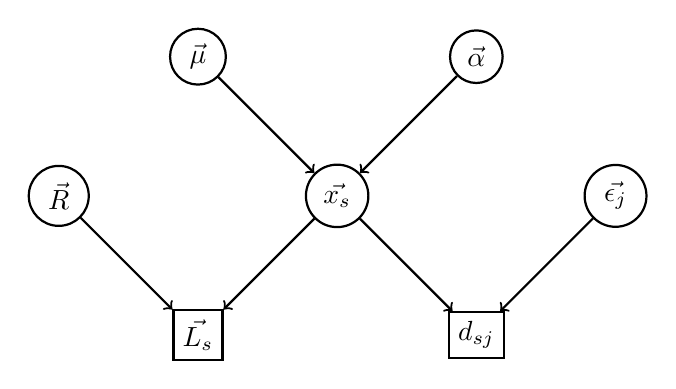
\begin{tikzpicture}[node distance={25mm}, thick, main/.style = {draw, circle}]
 			\node[main] (1) {$\vec{\boldmath{x_s}}$};
 			\node[main] (2) [above left of=1] {$\vec{\mu}$};
 			\node[main] (3) [above right of=1] {$\vec{\alpha}$};
 			\node[draw] (4) [below right of=1] {$d_{sj}$};
 			\node[draw] (5) [below left of=1] {$\vec{L_s}$};
 			\node[main] (6) [above right of=4] {$\vec{\epsilon_j}$};
 			\node[main] (7) [above left of=5] {$\vec{R}$};

 			\draw[->] (2) -- (1);
 			\draw[->] (3) -- (1);
 			\draw[->] (1) -- (4);
 			\draw[->] (1) -- (5);
 			\draw[->] (6) -- (4);
 			\draw[->] (7) -- (5);
 		\end{tikzpicture}
 		\caption{Potential DAG of the model.}
 		\label{fig:DAG_model}
 	\end{figure}
%
%
% 	\subsection{LOTUS database}
% 	Since LOTUS database \cite{rutzLOTUSInitiativeOpen2022} has no properties in $\vec{c}$ other than species and molecules, we denote
% 	 $$P(\vec{L_S} | \vec{x_s}, \vec{R}) = P(\vec{L_s} | \vec{\xi_s}, \vec{R}), $$
% 	 with $\vec{\xi_s} = (\xi_{s1}, \ldots, \xi_{sM} )$ the vector of presence/absence of all molecules $M$ in species $s$. Furthermore, $\xi_{sm} = min(1, \sum_{t}^{T} x_{smt})$ the minimum between $1$ and the sum of presence or absence of a molecule across all tissues.
%
% 	 Based on the defined vectors in \cref{subsec:definition}, we can assume a more general case with :
%
% 	 \begin{equation}
% 	 	\xi_{sm} = min\left[1, \sum_{k=1}^{K} \sum_{l=1}^{L_k} x_{smw_{k_l}} \right] \quad,
% 	 \end{equation}
%
%  The probability of having a molecule present in the LOTUS database not only depends on the presence/absence of that molecule in a species but also on the research effort done for a specific molecule or species. We thus have $R_{sm} = f(n_s, n_m)$ with $R_{sm} \in [0,1]$ and where $n_s$ and $n_m$ are the number of scientific papers that relate respectively the species or the molecules of interest. We thus have the following matrix : \\
%
%  \begin{blockarray}{cccc}
%  	& $L_{sm} = NA$ & $L_{sm} = 1$ \\
%  	\begin{block}{c(ccc)}
%  		$x_{sm}=0$ & $1$ & $0$  \\
%  		$x_{sm}=1$ & $1-R_{sm}$ & $R_{sm}$ \\
%  	\end{block}
%  \end{blockarray}
%
%
% 	\subsection{MS data}
% 	Let $\vec{d_{sj}}=(d_{sj1}, \ldots, d_{sjM})$ be the presence-absence vector of each metabolite $m$ obtained with mass-spectrometry run $j=1,\ldots,J_s$ performed on species $s$. Assuming a false-positive and false-negative error rates $\epsilon_{01}$ and $\epsilon_{10}$, respectively, we have
%
% 	\begin{equation*}
% 		\P(\d_{sj}|\x, \epsilon_{01}, \epsilon_{10}) = \prod_m \left[ x_{sm}\left(\epsilon_{10}^{1-d_{sjm}}(1-\epsilon_{10})^{d_{sjm}}\right) + (1-x_{sm})\left( \epsilon_{01}^{d_{sjm}}(1-\epsilon_{01})^{1-d_{sjm}}\right)\right].
% 	\end{equation*}





\section{v2}
We seek to infer the presence or absence of metabolites in group of samples compartmentalized by $T$ of discrete axes such as e.g. species, tissue or environmental conditions. For any compartment $c$, let $\tau_t(c) = 1, \ldots, n_t$ indicate the compartment index along axis $t=1, \ldots, T$. For convenience, let us further denote by $\tau_\M(c)$ and $\tau_\S(c)$ the metabolite and species of that compartment.

Let $x_{c}$ denote the presence ($x_c=1$) or absence ($x_c=0$) of a metabolite $\tau_\M(c)$ in compartment $c$ and let $\x=(x_1, \ldots, x_C)$ be the full vector $x_c$ across all compartments $c=1, \ldots, C$ with $C=\prod_t n_t$.

We will assume that similarities across any of the axis of compartmentalization is reflected in the patterns of presences and absences in $\x$. For instance, closely related species may share a similar set of metabolites and  metabolites related in their synthesis may share a similar distribution across species. To model such similarities, we assume that the probability $\P(x_c=1|\bmu_c, \epsilon_c)$ with which metabolite $\tau_\M(c)$ is present in compartment $c$ is given by

\begin{equation}
	\logit \P(x_c=1|\bmu_c, \epsilon_c) = \sum_{t=1}^{T} \mu^{(t)}_{\tau_t(c)} + \epsilon_{c}
\end{equation}

where $\bmu_c=(\mu^{(1)}_{\tau_1(c)}, \ldots, \mu^{(T)}_{\tau_T(c)})$ is a vector of axis specific intercepts and $\epsilon_{c}$ is normally distributed with mean 0 and co-variance

\begin{equation}
	\cov(\epsilon_c, \epsilon_{c'}) = \sum_t \beta^{(t)}_{\tau_t(c)} + \sum_t \beta^{(t)}_{\tau_t(c')} + \prod_t \prod_{f=1}^{F_t} \sigma_{tf}\Big(\tau_t(c), \tau_t(c')\Big)^{\alpha_{tf}}
\end{equation}



Here, the $\beta^{(t)}_{\tau_t(c)}$ are positive intercepts specific for the compartment index $\tau_t(c)$ along axis $t$, the $\sigma_{tf}, f=1, \ldots, F_t,$ are the $F_t$ known covariance matrices between entries along axis $t$, and the $\alpha_{tf}$ are positive scalars.

\subsection{Emission probabilities}

We consider several different types of data to inform about $\x$. This data may be of different dimensionality, e.g. may only discriminate along a subset of the axes or at a higher scale along some axes. For a particular data set $d=1, \ldots, D$, let $\bxi_d=\{\xi_{d1}, \ldots, \xi_{du}\}$ denote the sets of distinguished compartments. We then define the presence of ($\x(\xi_{du})=1$) or absence ($\x(\xi_{du})=0$) in set $\xi_{du}, u=1\ldots,U,$ as

\begin{equation*}
 \x(\xi_{du}) = \min \left(1, \sum_{c \in \xi_{du}} x_c \right).
\end{equation*}


\subsubsection{LOTUS}

 The LOTUS database \cite{rutzLOTUSInitiativeOpen2022} lists known occurrences of metabolites in species. Let $L_{ms} = 1$ denote a known occurrence of metabolite $m$ in species $s$, while $L_{ms}=0$ denotes that no evidence for such an occurrence has been reported, either because the metabolite $m$ is truly absent in species $s$ or because of a lack of research effort.

 Let us denote by $R_{sm}$ the probability of discovery of metabolite $m$ in species $s$ such that
 \begin{equation*}
  \P(L_{ms}|\x(\xi(m,s)), R_{ms}) = \begin{cases}
                             0 \quad &\mathrm{if\ } \x(\xi(m,s))=0 \mathrm{\ and\ } L_{ms} = 1,\\
                             1 \quad &\mathrm{if\ } \x(\xi(m,s))=0 \mathrm{\ and\ } L_{ms} = 0,\\
                             R_{ms} \quad &\mathrm{if\ } \x(\xi(m,s))=1 \mathrm{\ and\ } L_{ms} = 1,\\
                             1- R_{ms} \quad &\mathrm{if\ } \x(\xi(m,s))=1 \mathrm{\ and\ } L_{ms} = 0,
                            \end{cases}
 \end{equation*}

 where $\xi(m,s)$ is the set of compartments relevant for metabolite $m$ and species $s$, i.e. all compartments $c$ for which $\tau_\M(c)=m$ and $\tau_\S(c)=s$.

 To quantify the research effort $R_{ms}$ of a particular entry $L_{ms}$, we will rely on two measures, the total number of relevant papers published for metabolite $m$ ($P_m$) and for species $s$ ($Q_s$), such that

 \begin{equation*}
 R_{ms} = 1 - e^{-\gamma P_m - \delta Q_s}
 \end{equation*}
with positives scalars $\gamma$ and $\delta$.


\subsection{Prior distributions}

\begin{itemize}
 \item $\mu_{ti} \sim \N(0, \sigma^2_\mu), t=1, \ldots, T, i=1\ldots, n_t$ with $\sigma^2_\mu=1$
 \item $\alpha^{(t)}_f \sim \Exp(\lambda_\alpha), t=1, \ldots, T, f=1\ldots, F_t$
 \item $\beta^{(t)}_i \sim \Exp(\lambda_\beta), t=1, \ldots, T, i=1\ldots, n_t$
 \item $\gamma \sim \Exp(\lambda_\gamma)$
 \item $\delta \sim \Exp(\lambda_\delta)$
\end{itemize}


\subsection{Simulations}

\begin{itemize}
 \item Simulate $P_m$ and $Q_s$ from a Poisson distribution
 \item Simulate $\sigma_{tf}$ using a Wishart distribution (?)
\end{itemize}



\bibliographystyle{unsrturl}
\bibliography{/Users/Marco/BibTex/BibTex}

\end{document}
